\section{Use Case Diagrams}

A Use Case diagram is ``a definition of a meaningful interaction with a 
computer system'' \citep{lunn03}. Use case diagrams are a powerful analysis 
technique. At the highest level they can easily define the presentation of a
system, whilst at the most detailed level can fully specify the external 
functionality of a system.

Within this section the use case of the entire system will be explored in 
detail. Figure \ref{fig:use_case} shows the use case for the entire system. 

To simplify the diagram, certain extensions and inclusions have been omitted. 
In the following sections these are discussed in more detail below.

\begin{figure}[H]
  \centering
    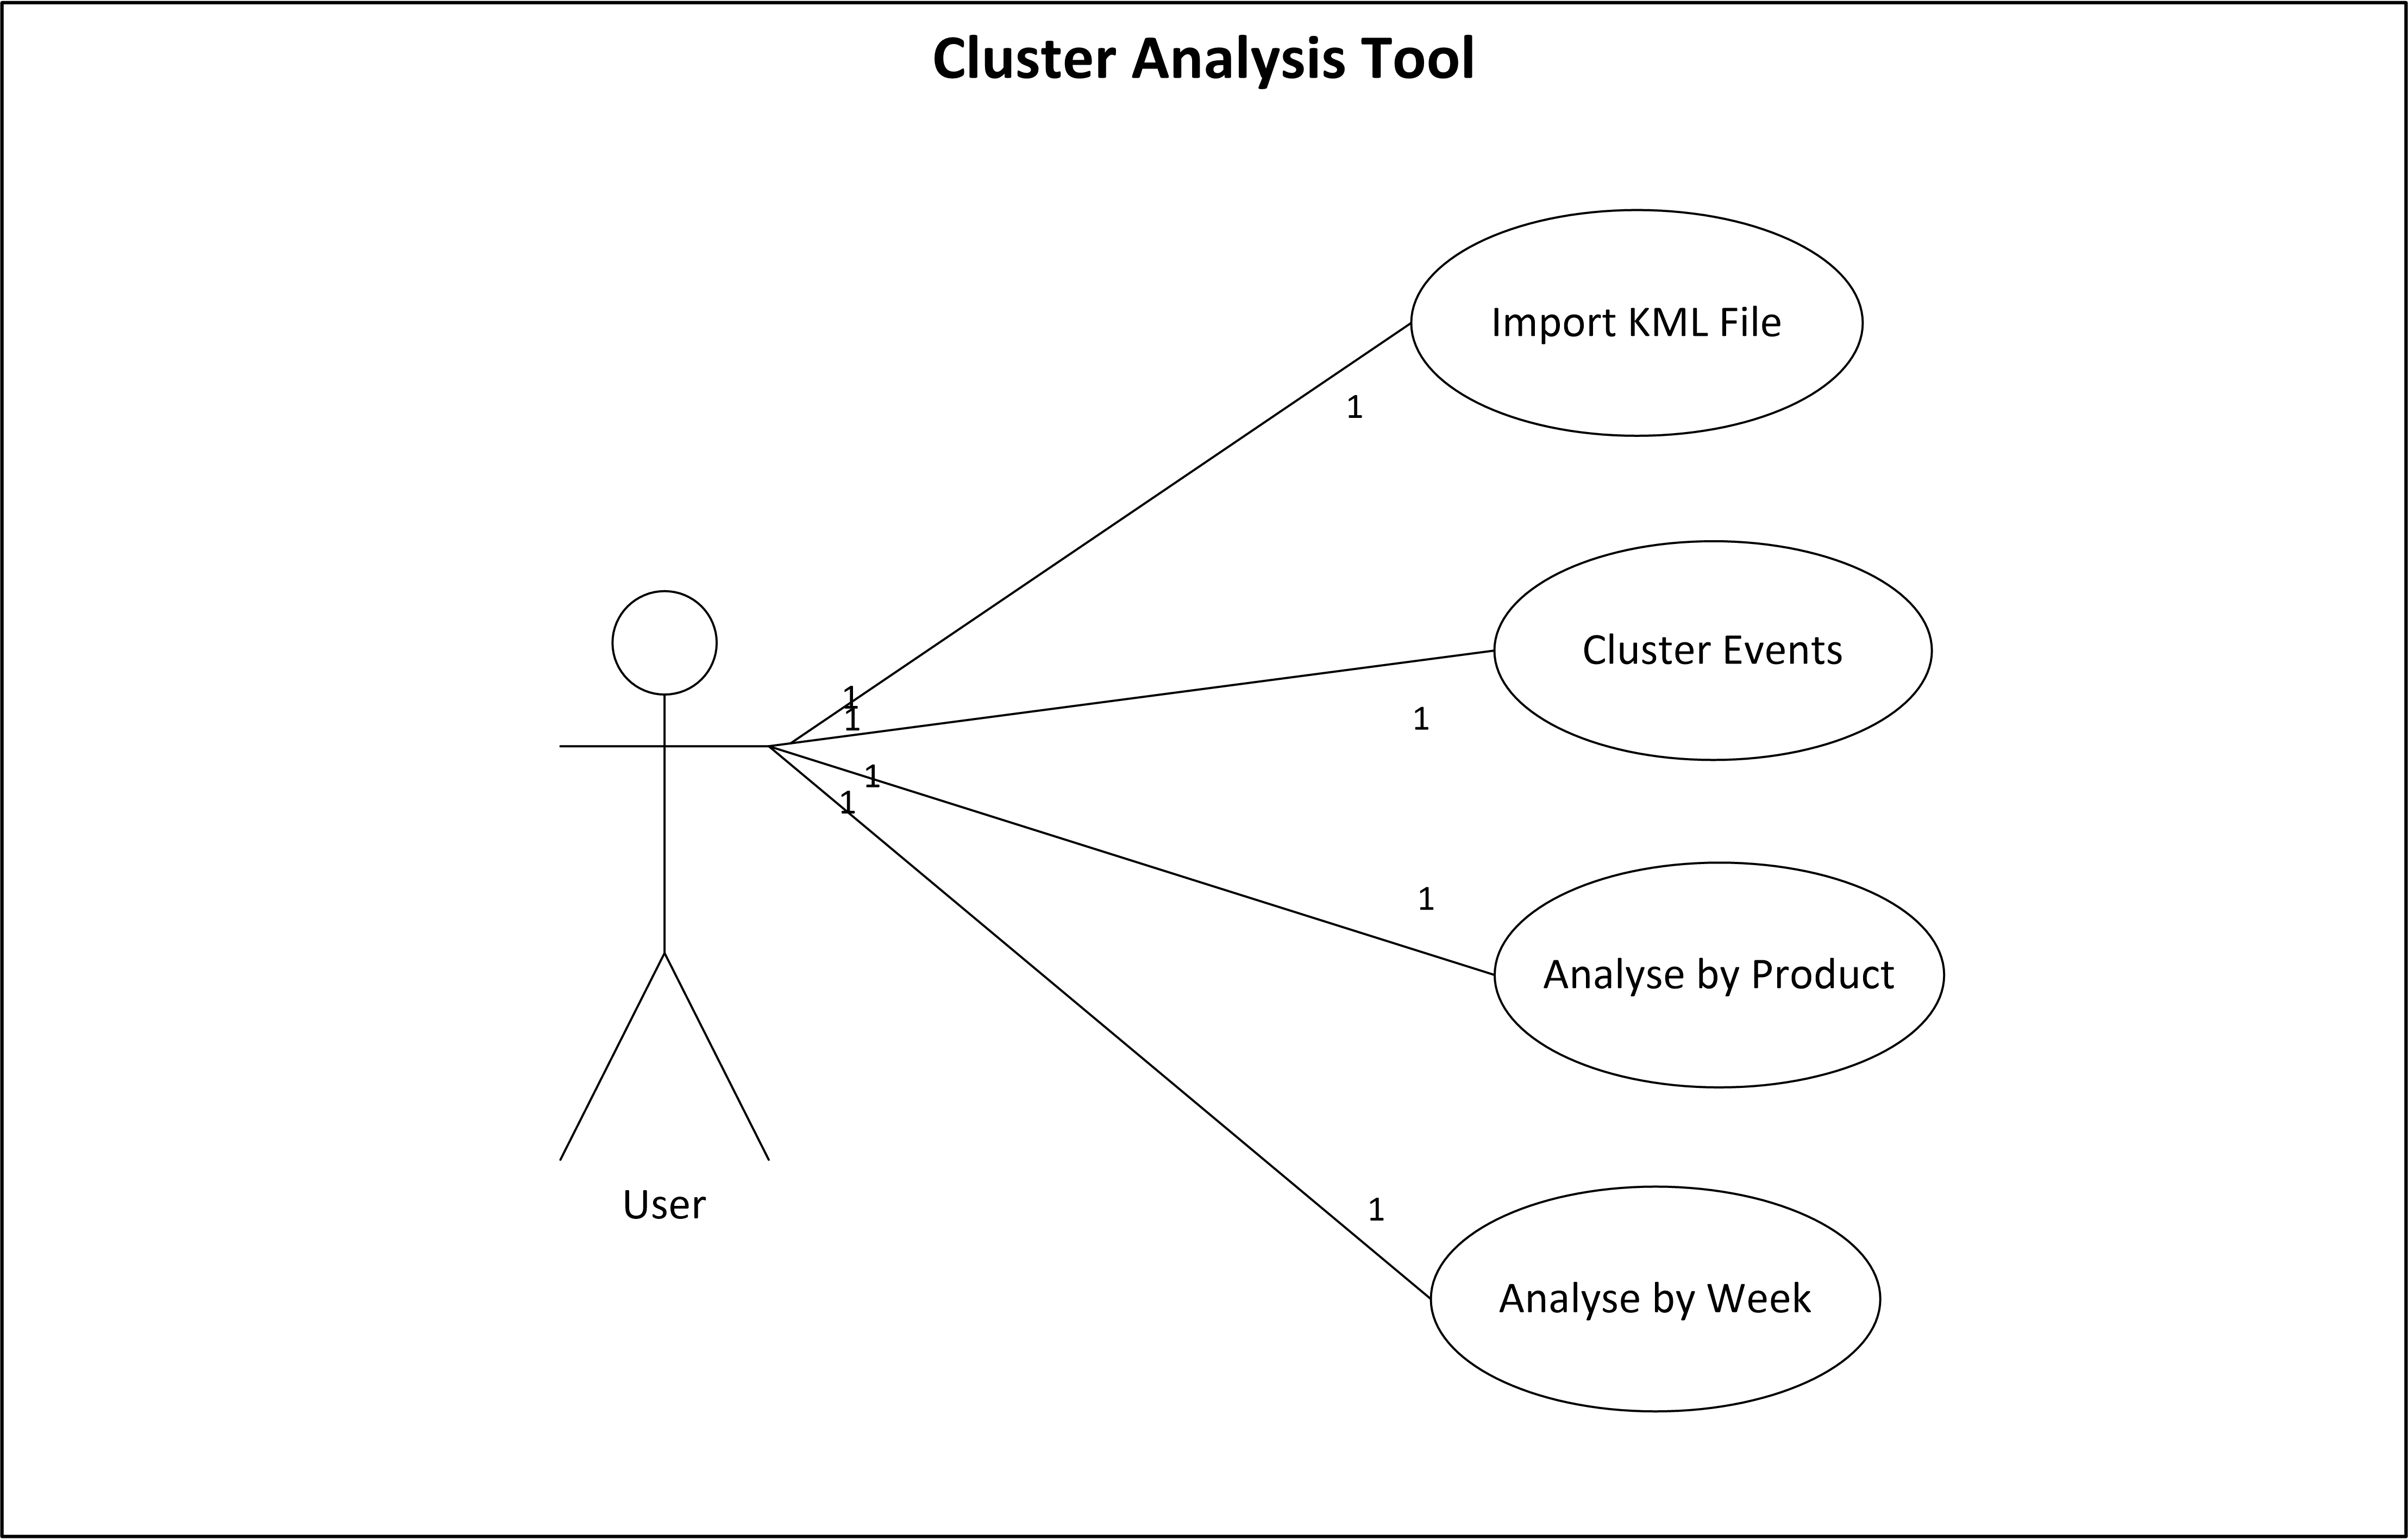
\includegraphics[scale=0.9]{chapter7/use_case/use_case.png}
    \caption[Use case diagram of the entire system]
            {Use case diagram of the entire system}
    \label{fig:use_case}
\end{figure}


\subsection{Importing Data}
Figure \ref{fig:UCImportData} highlights the use case for importing data into 
the system. The user is able to request that the tool imports either a single 
KML file or a directory containing multiple KML files.

The addition of this small option allows the end user to perhaps select various 
files that are stored across the file system. It also allows the user to point 
the tool directly at a directory that contains the required KML files.

Although integration with BlackBerry internal systems was originally a 
requirement that would not be implemented, this small addition does allow 
easier integration with any existing systems.

\begin{figure}[H]
  \centering
    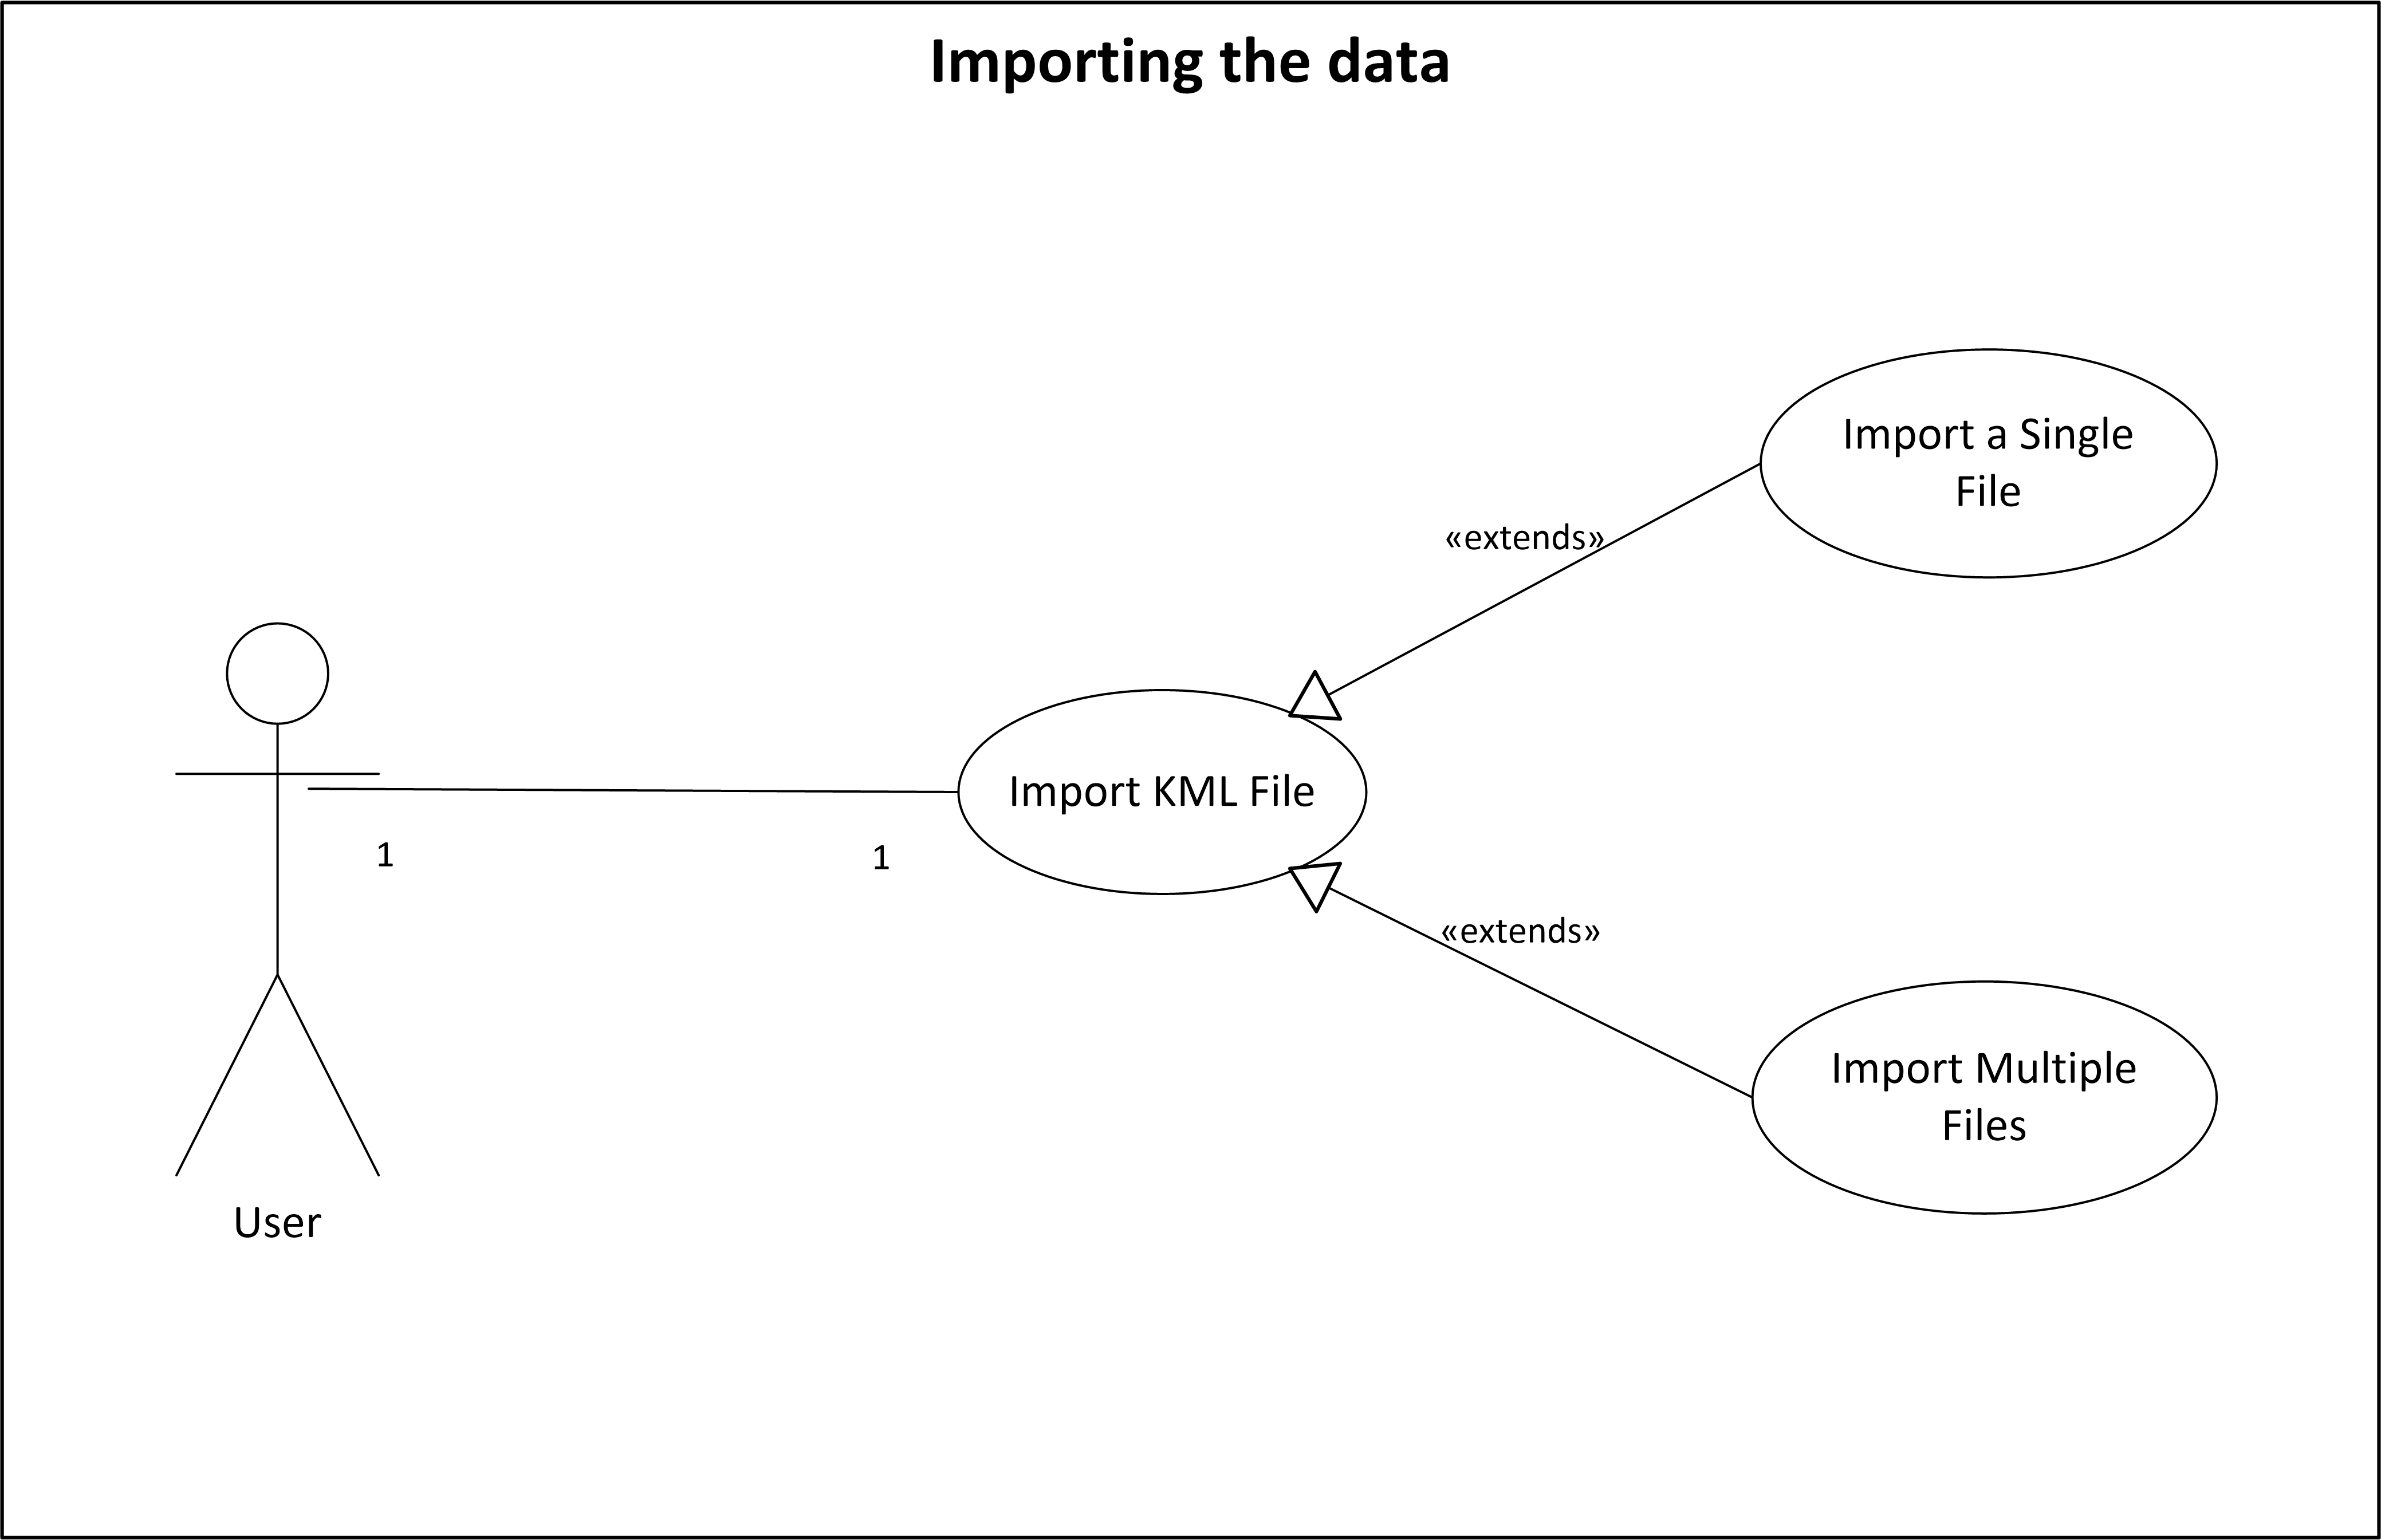
\includegraphics{chapter7/use_case/importing_data.png}
    \caption[Use case diagram to import KML data]
            {Use case diagram to import KML data}
    \label{fig:UCImportData}
\end{figure}


\subsection{Clustering}
Figure \ref{fig:UCClusterData} highlights the use case for clustering the data. 
In order to cluster, it is assumed that the user has already given a set of 
data to the algorithm.

The clustering mechanism utilises the DBSCAN algorithm, and requires two 
additional parameters in order to complete the clustering process. 

Firstly the algorithm will require a minimum number of points. This is the 
minimum number of points (or objects) required to form a cluster. This value 
must be set by the user, otherwise a default value will be used.

Secondly the algorithm will require the {\em EPS} value. The {\em EPS} 
(epsilon) value is the maximum distance allowed between two points (or objects)
to form a cluster.

\begin{figure}[H]
  \centering
    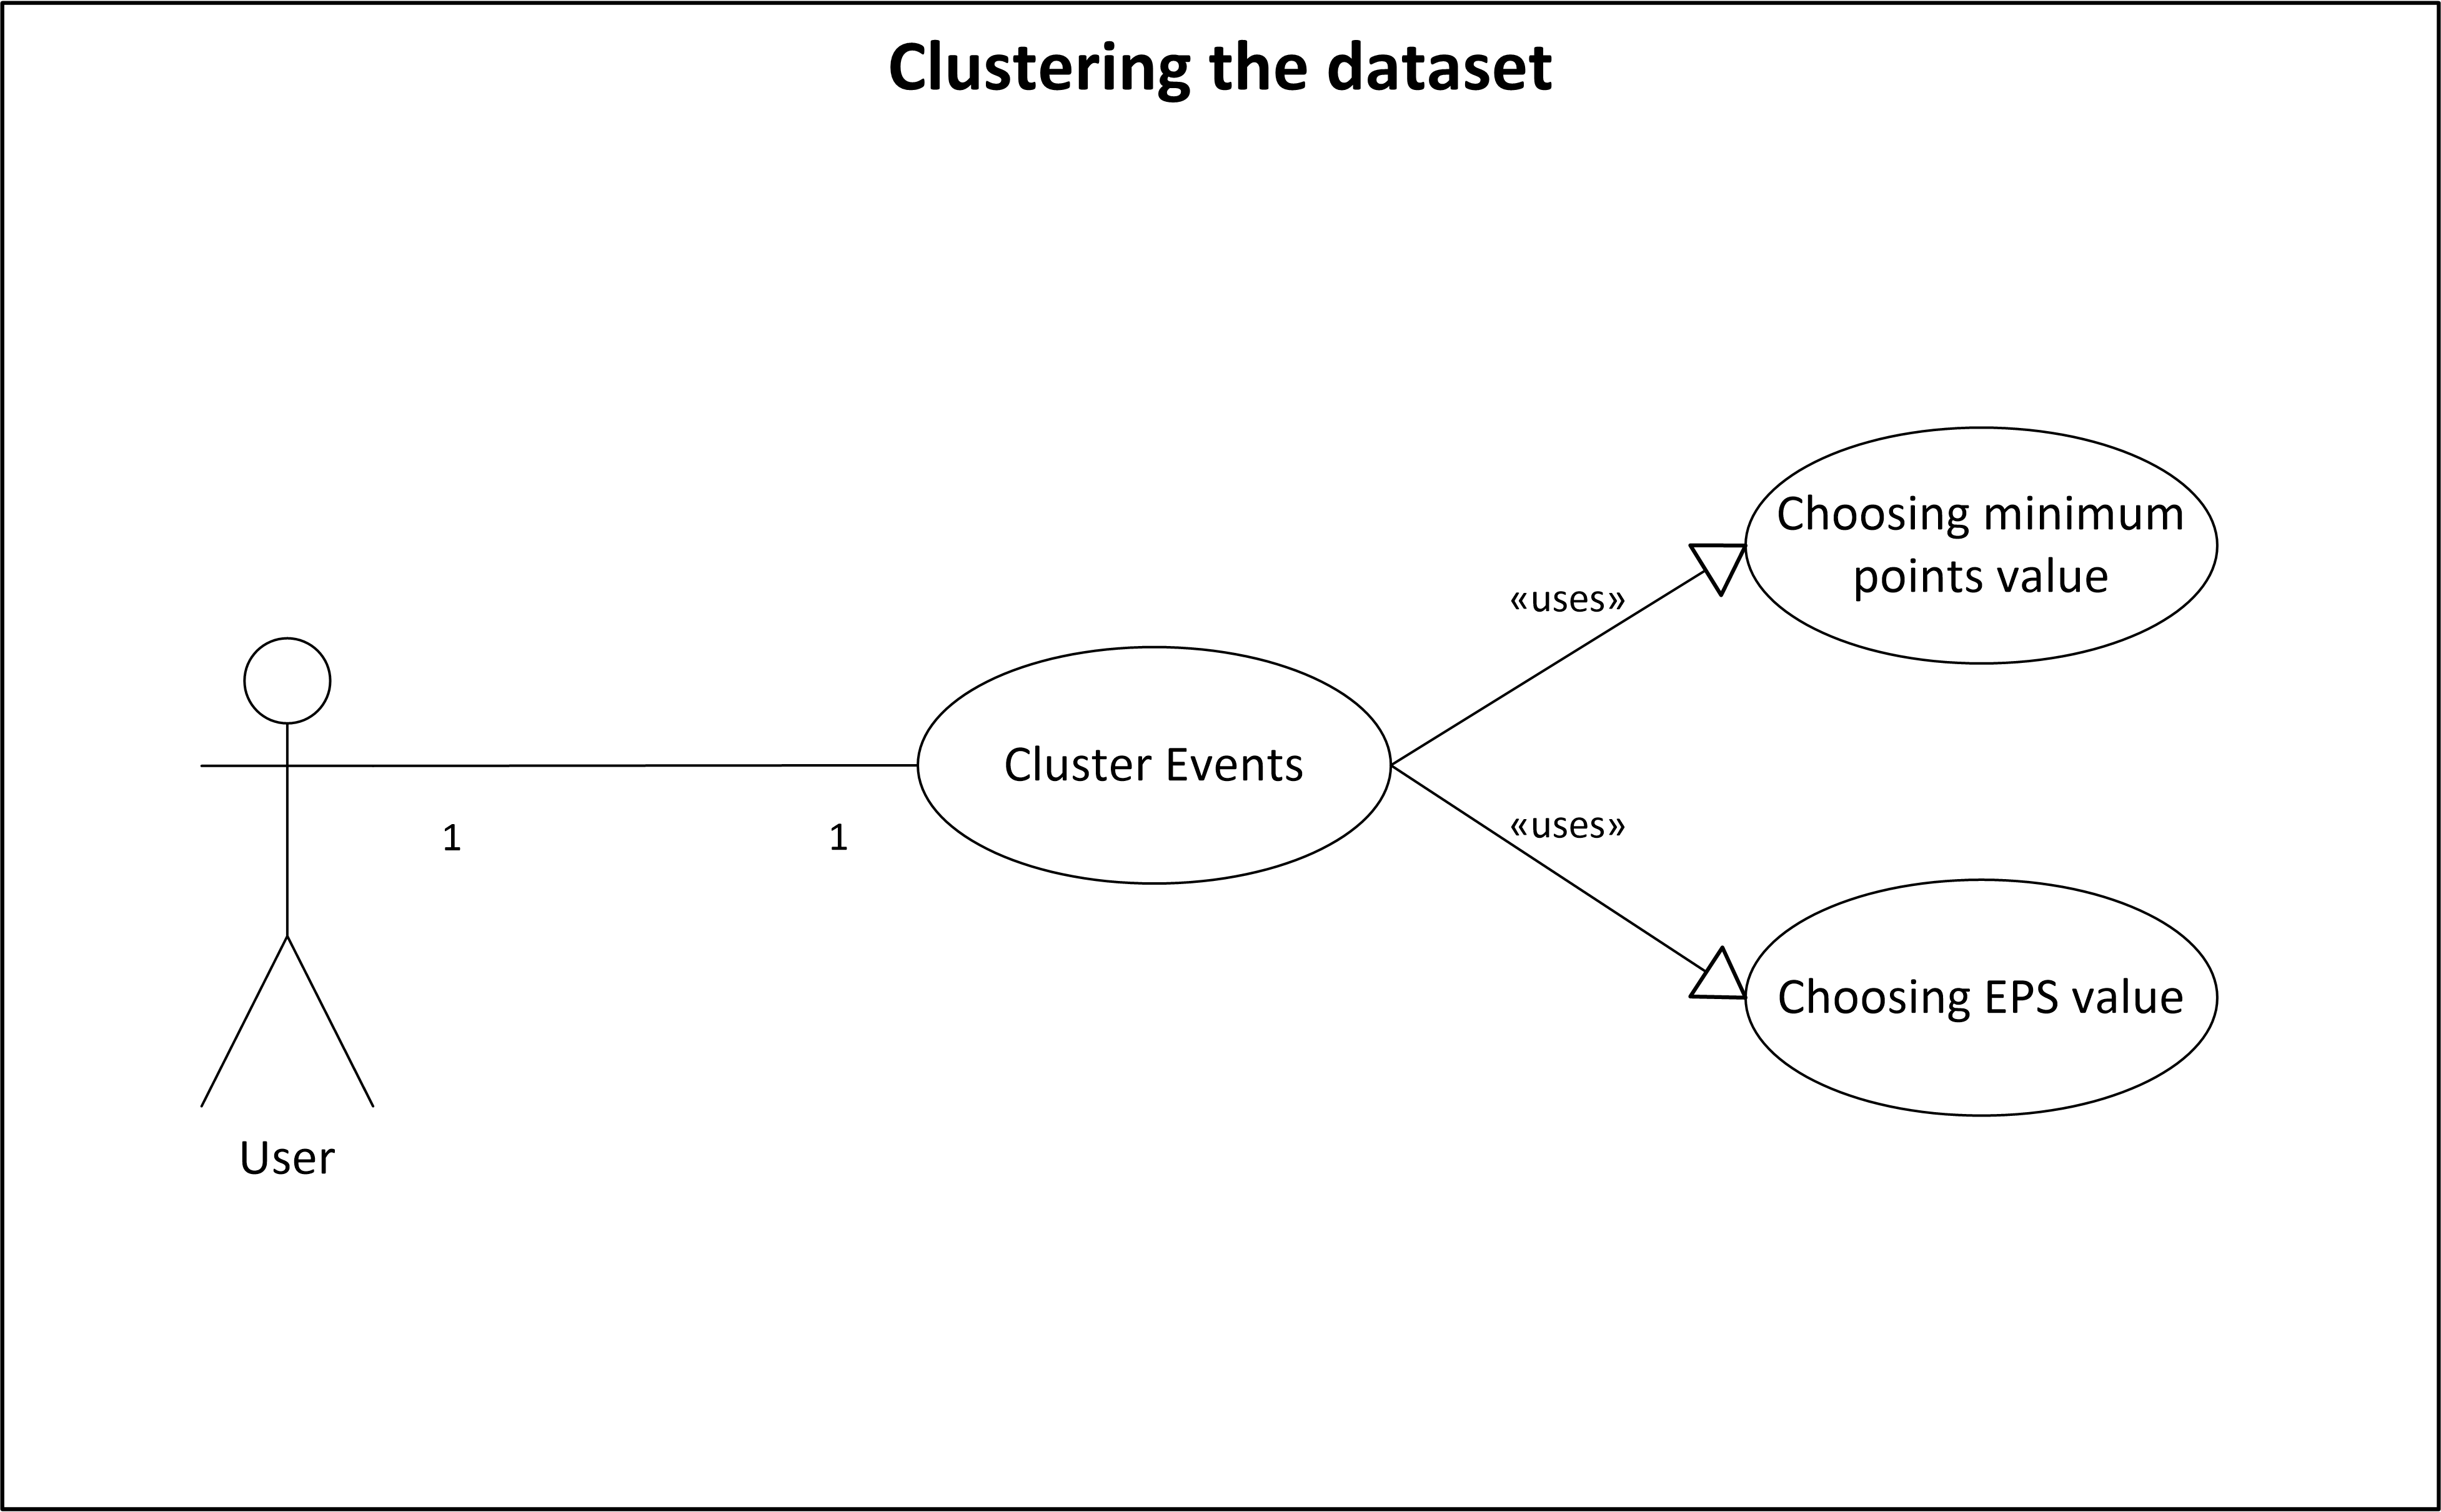
\includegraphics{chapter7/use_case/cluster_data.png}
    \caption[Use case diagram highlighting data clustering]
            {Use case diagram highlighting data clustering}
    \label{fig:UCClusterData}
\end{figure}


\subsection{Results Analysis}
Figure \ref{fig:UCAnalyseData} highlights the use case for analysing the 
clustered data. Fundamentally, the analysis of clusters can take two distinct 
paths. Analysis can happen upon a Weekly basis or a Product basis.

Regardless of whichever fundamental route was taken, the back end analysis is 
the same. Firstly the user could create a number of charts that highlights the 
differences in RAT, Mix-Band and Start RRC state usages, as well as cluster 
sizes.

Secondly, the user could create a KML file, that is able to be view from within
Google Earth. This would show each cluster upon a map, along with a heat map to 
highlight the cluster intensities.

Finally use user could choose to create a number of charts, and create an 
output KML file --- i.e. perform both of the previous options.

\begin{figure}[H]
  \centering
    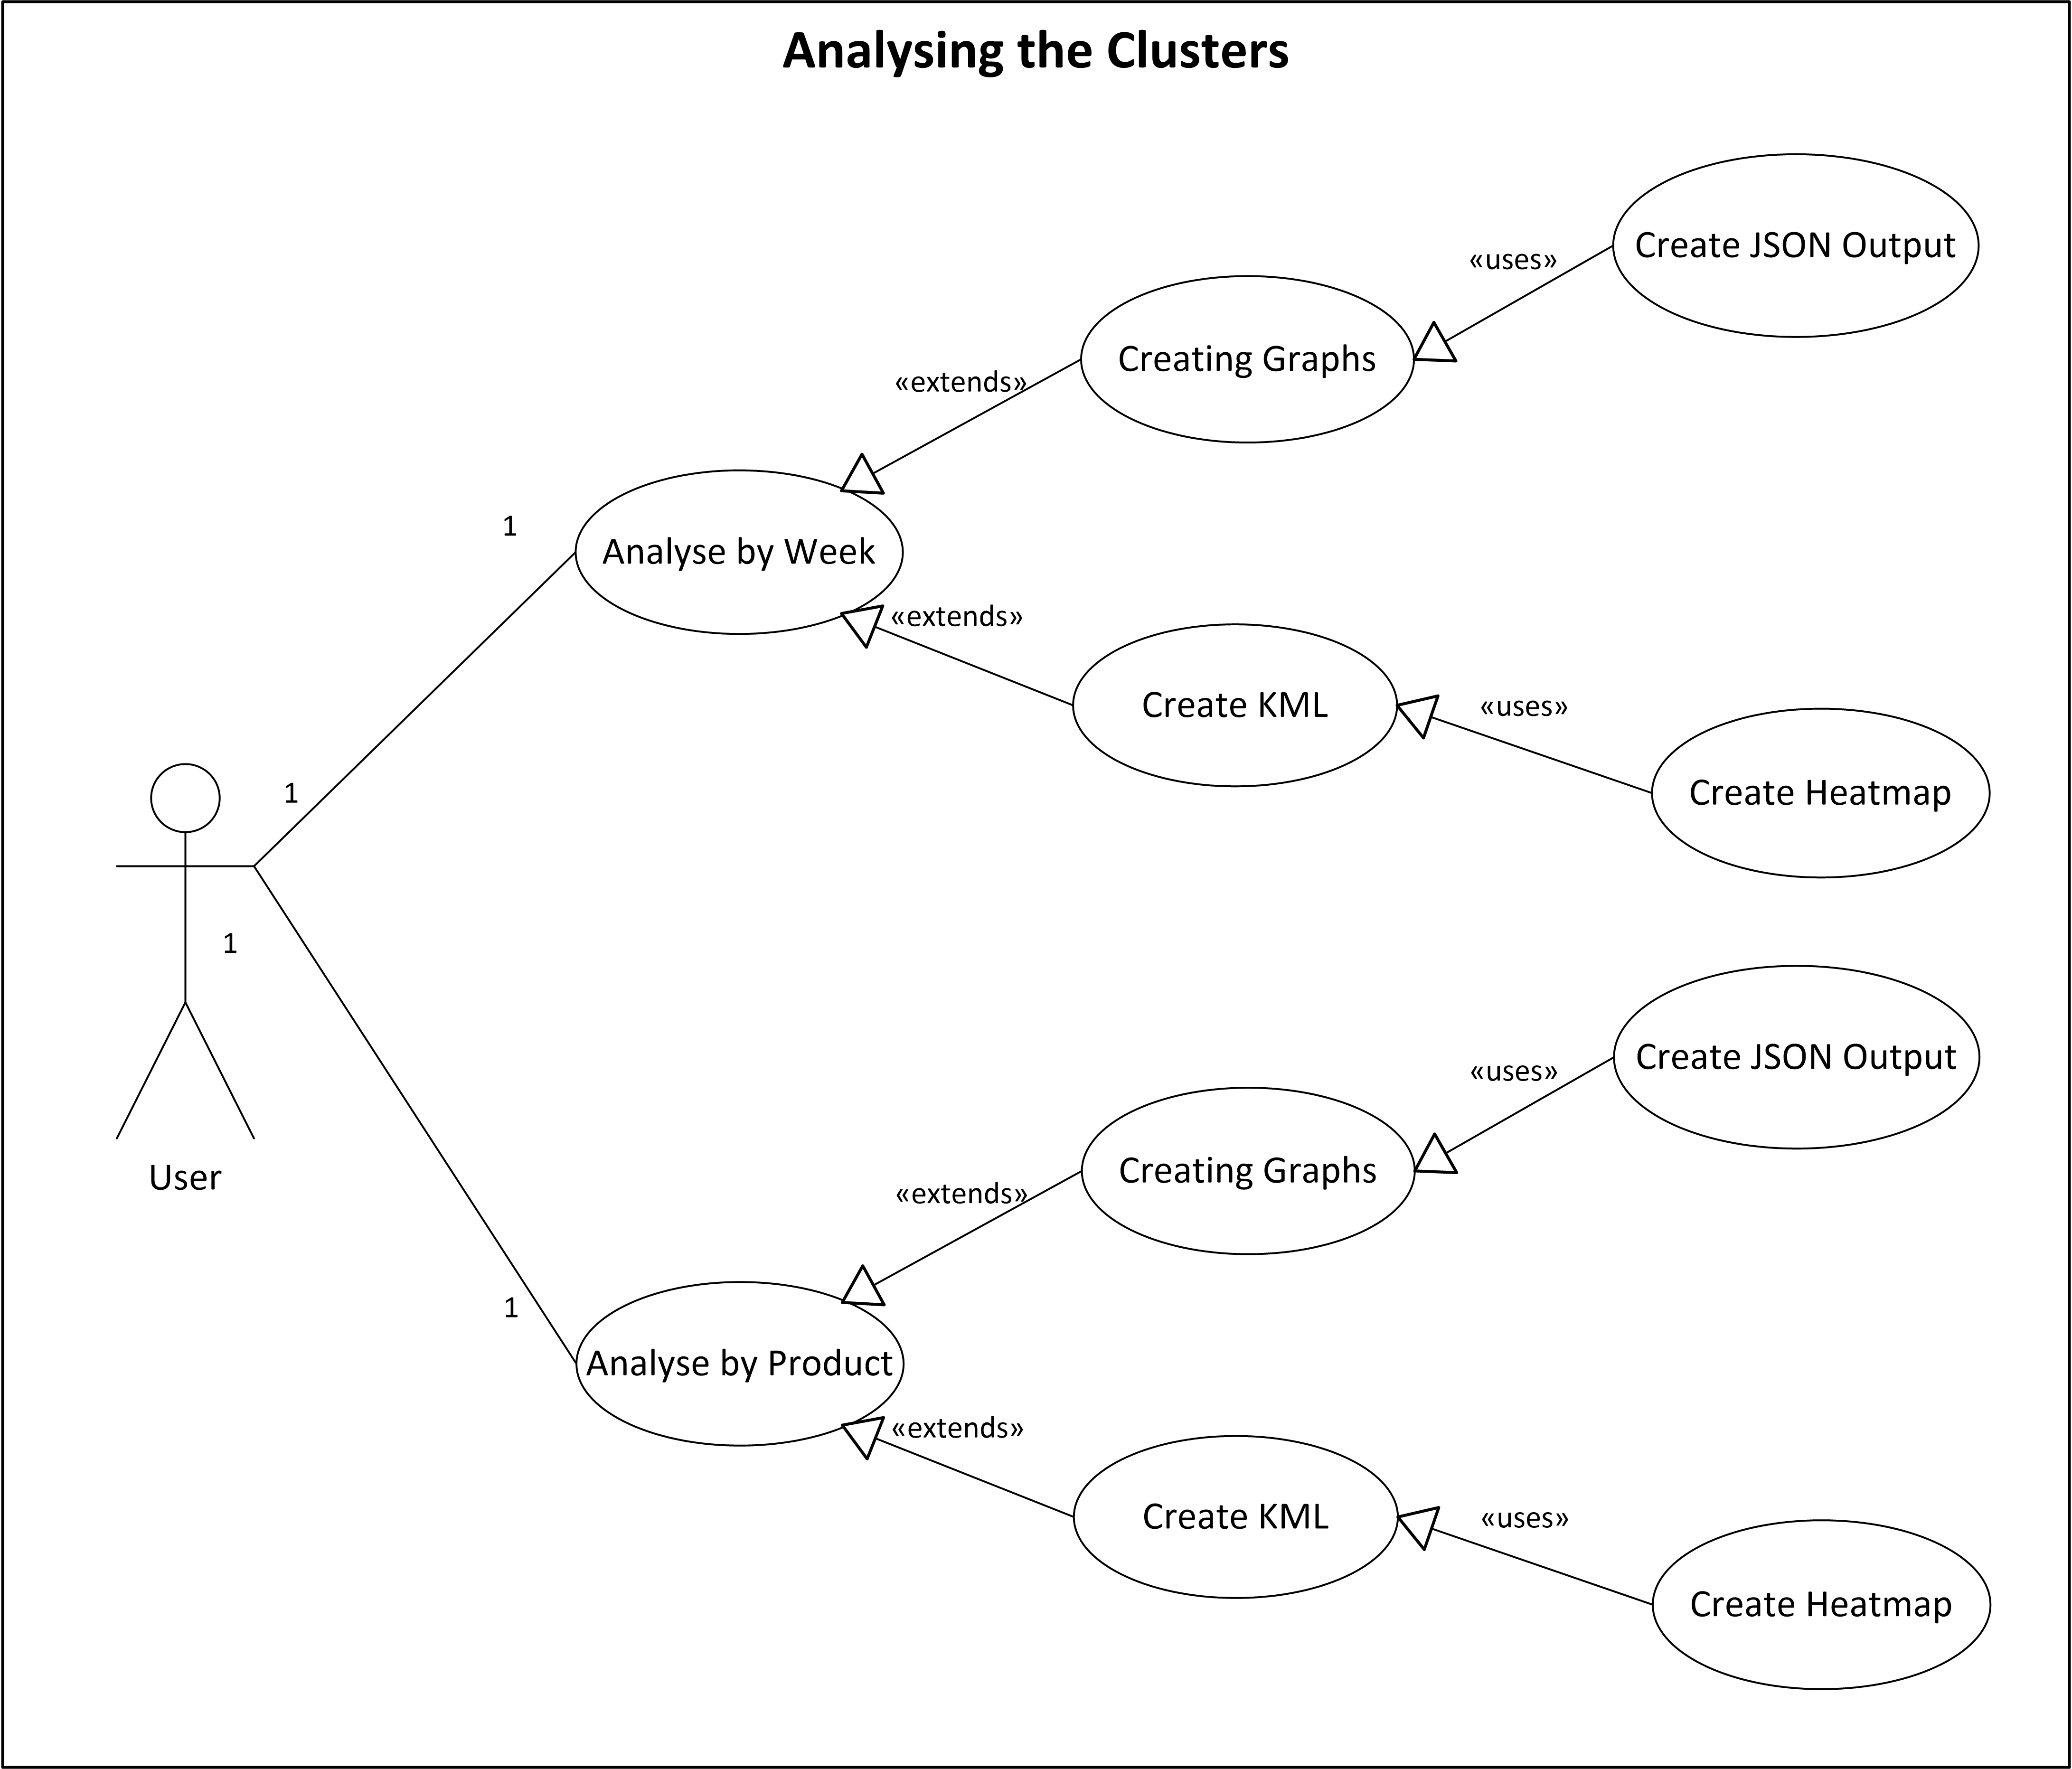
\includegraphics{chapter7/use_case/analyse_results.png}
    \caption[Use case diagram highlighting importing data]
            {Use case diagram highlighting importing data}
    \label{fig:UCAnalyseData}
\end{figure}
